\documentclass{article}

%% Page Margins %%
\usepackage{geometry}
\geometry{
    top = 0.75in,
    bottom = 0.75in,
    right = 0.75in,
    left = 0.75in,
}

\usepackage{amsmath}
\usepackage{graphicx}
\usepackage{parskip}

\title{Lab 3: The Arithmetic Logic Unit}

% TODO: Enter your name
\author{Qianjun Huang}

\begin{document}
\maketitle

\section*{Part I}

\begin{enumerate}
\setcounter{enumi}{1}
\item Export the subcircuit schematic as an image and include it in your report.

\begin{figure}[ht!]
    \centering
    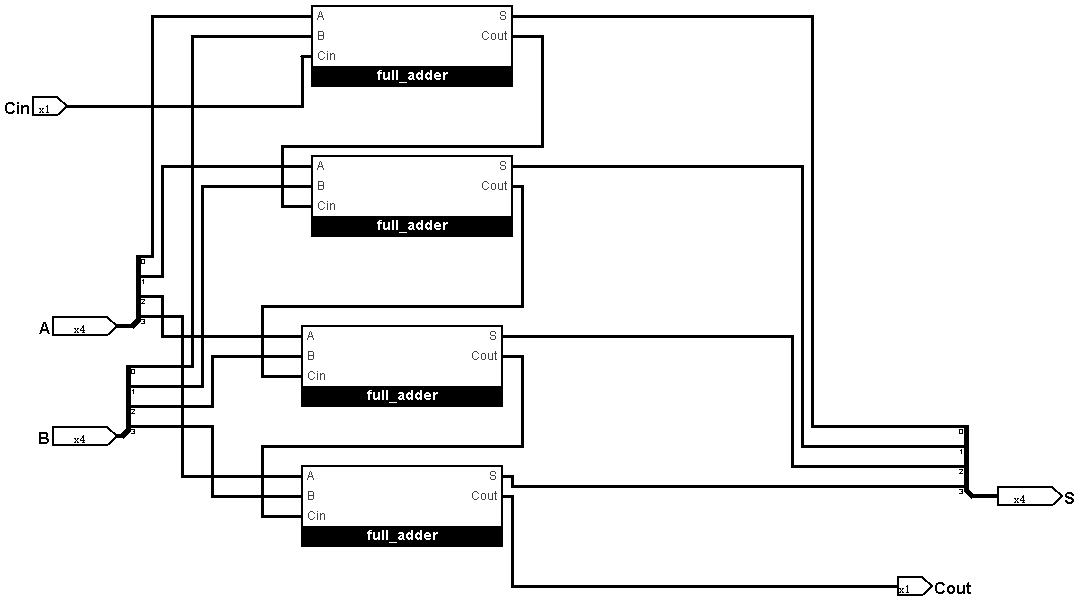
\includegraphics[width=0.6\textwidth]{lab3_part1.png}
    \caption{A schematic of ripple\_carry4.}
    \label{f:part1}
\end{figure}

\item Include a screenshot of your simulated test vector for the 4-bit Ripple Carry Adder.

\begin{figure}[ht!]
    \centering
    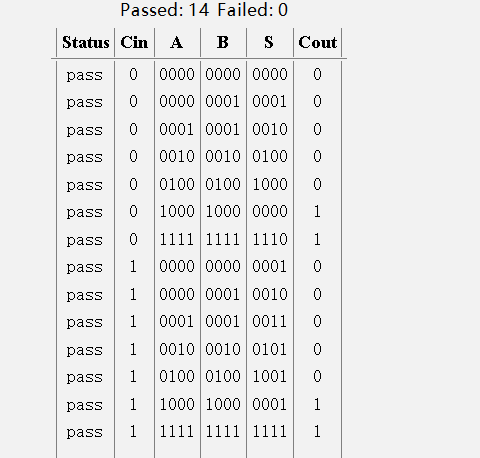
\includegraphics[width=0.4\textwidth]{lab3_part1_simulation.png}
    \caption{A simulation ripple\_carry4.}
    \label{f:part1_simulation}
\end{figure}
\end{enumerate}

\section*{Part II}

\begin{enumerate}
\item Export the subcircuit schematic of each operation as an image and include it in your report.

\begin{figure}[ht!]
    \centering
    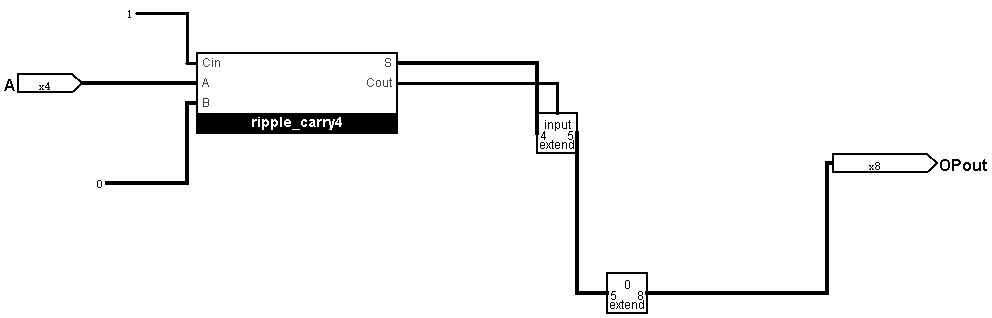
\includegraphics[width=0.4\textwidth]{lab3_op0.png}
    \caption{A schematic of op0.}
    \label{f:op0}
\end{figure}

\begin{figure}[ht!]
    \centering
    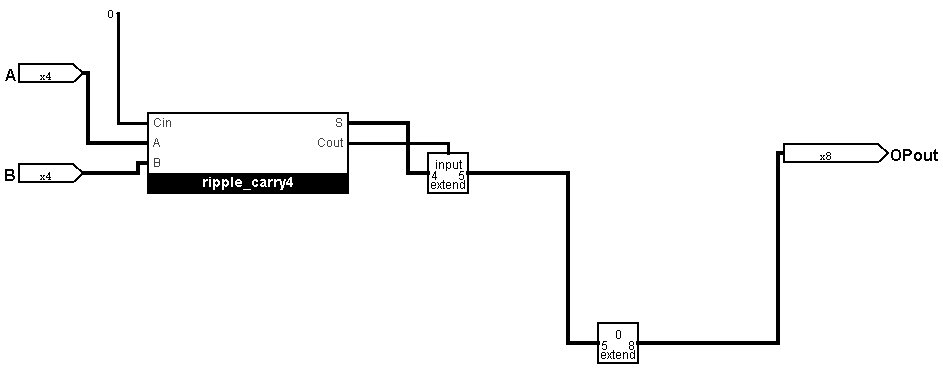
\includegraphics[width=0.4\textwidth]{lab3_op1.png}
    \caption{A schematic of op1.}
    \label{f:op1}
\end{figure}

\begin{figure}[ht!]
    \centering
    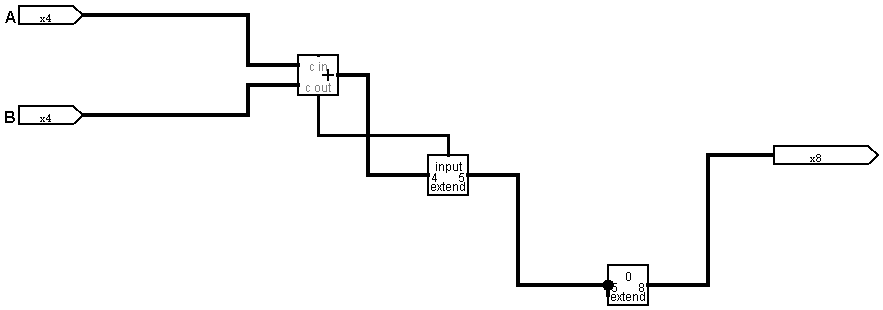
\includegraphics[width=0.4\textwidth]{lab3_op2.png}
    \caption{A schematic of op2.}
    \label{f:op2}
\end{figure}

\begin{figure}[ht!]
    \centering
    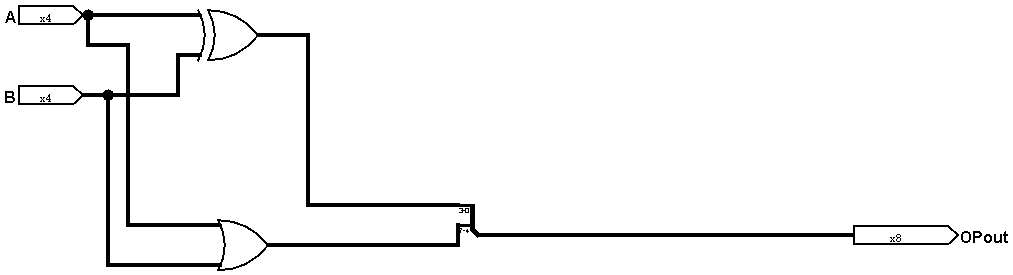
\includegraphics[width=0.4\textwidth]{lab3_op3.png}
    \caption{A schematic of op3.}
    \label{f:op3}
\end{figure}

\begin{figure}[ht!]
    \centering
    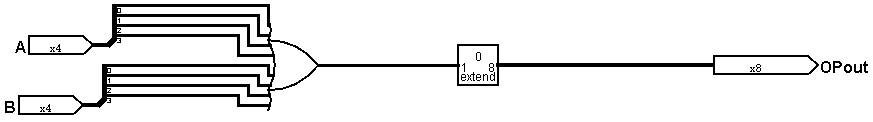
\includegraphics[width=0.4\textwidth]{lab3_op4.png}
    \caption{A schematic of op4.}
    \label{f:op4}
\end{figure}

\begin{figure}[ht!]
    \centering
    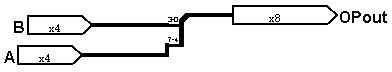
\includegraphics[width=0.4\textwidth]{lab3_op5.png}
    \caption{A schematic of op5.}
    \label{f:op5}
\end{figure}

\item Include a screenshot of your simulated test vectors for op3, op4, and op5.

\begin{figure}[ht!]
    \centering
    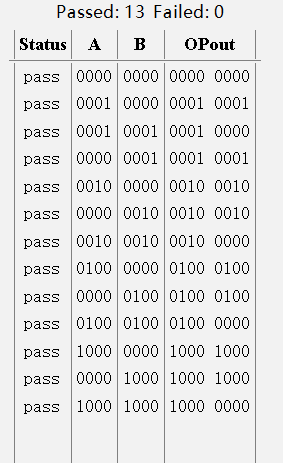
\includegraphics[width=0.4\textwidth]{lab3_op3_simulation.png}
    \caption{A simulation of op3.}
    \label{f:op3_simulation}
\end{figure}

\begin{figure}[ht!]
    \centering
    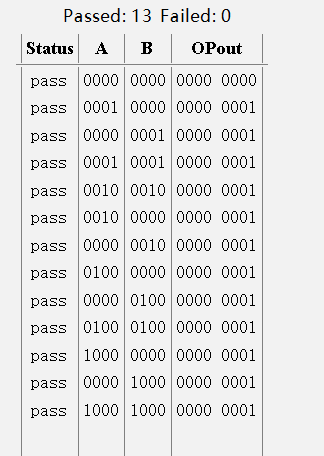
\includegraphics[width=0.4\textwidth]{lab3_op4_simulation.png}
    \caption{A simulation of op4.}
    \label{f:op4_simultion}
\end{figure}

\begin{figure}[ht!]
    \centering
    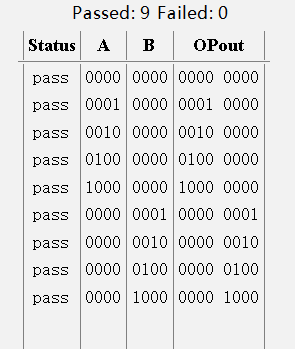
\includegraphics[width=0.4\textwidth]{lab3_op5_simulation.png}
    \caption{A simulation of op5.}
    \label{f:op5_simulation}
\end{figure}

\item Export the ALU schematic as an image and include it in your report.

\begin{figure}[ht!]
    \centering
    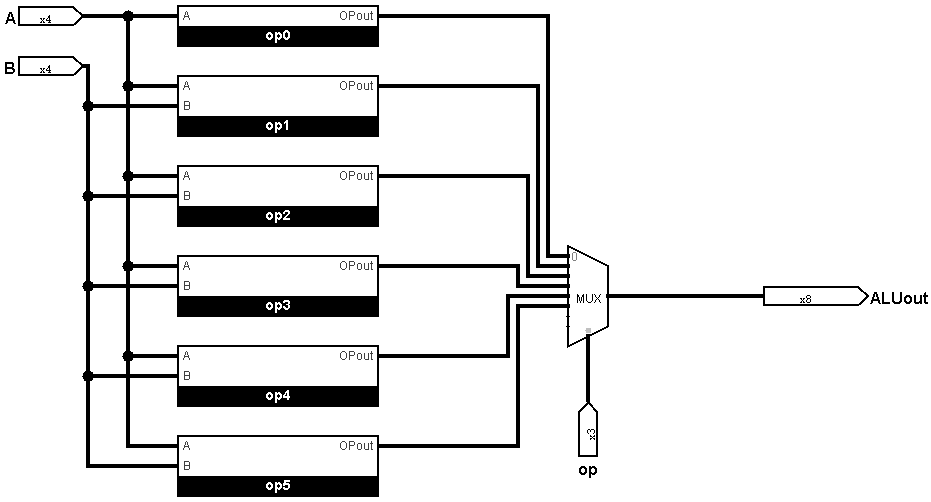
\includegraphics[width=0.6\textwidth]{lab3_alu.png}
    \caption{A schematic of the ALU.}
    \label{f:alu}
\end{figure}
\end{enumerate}

\end{document}